% Created by tikzDevice version 0.12.3.1 on 2021-11-23 19:16:47
% !TEX encoding = UTF-8 Unicode
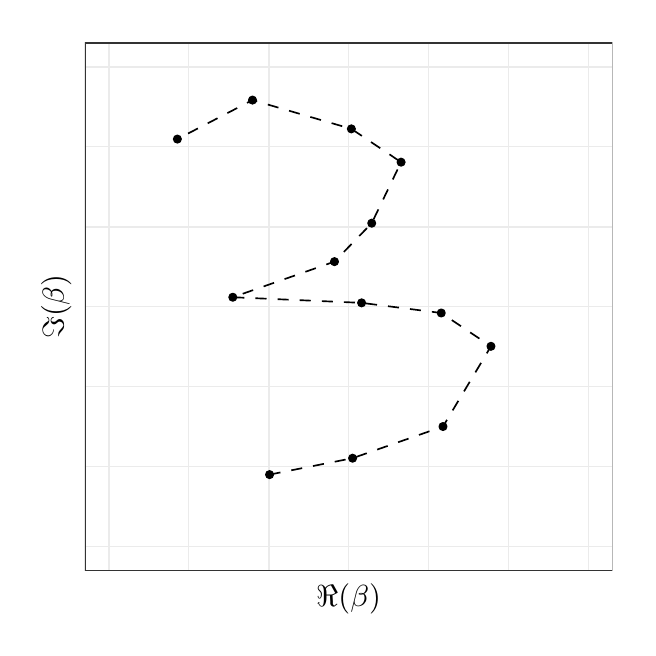
\begin{tikzpicture}[x=1pt,y=1pt]
\definecolor{fillColor}{RGB}{255,255,255}
\path[use as bounding box,fill=fillColor,fill opacity=0.00] (0,0) rectangle (216.81,216.81);
\begin{scope}
\path[clip] (  0.00,  0.00) rectangle (216.81,216.81);
\definecolor{drawColor}{RGB}{255,255,255}
\definecolor{fillColor}{RGB}{255,255,255}

\path[draw=drawColor,line width= 0.6pt,line join=round,line cap=round,fill=fillColor] (  0.00,  0.00) rectangle (216.81,216.81);
\end{scope}
\begin{scope}
\path[clip] ( 20.71, 20.71) rectangle (211.31,211.31);
\definecolor{fillColor}{RGB}{255,255,255}

\path[fill=fillColor] ( 20.71, 20.71) rectangle (211.31,211.31);
\definecolor{drawColor}{gray}{0.92}

\path[draw=drawColor,line width= 0.3pt,line join=round] ( 20.71, 58.26) --
	(211.31, 58.26);

\path[draw=drawColor,line width= 0.3pt,line join=round] ( 20.71,116.01) --
	(211.31,116.01);

\path[draw=drawColor,line width= 0.3pt,line join=round] ( 20.71,173.77) --
	(211.31,173.77);

\path[draw=drawColor,line width= 0.3pt,line join=round] ( 58.26, 20.71) --
	( 58.26,211.31);

\path[draw=drawColor,line width= 0.3pt,line join=round] (116.01, 20.71) --
	(116.01,211.31);

\path[draw=drawColor,line width= 0.3pt,line join=round] (173.77, 20.71) --
	(173.77,211.31);

\path[draw=drawColor,line width= 0.6pt,line join=round] ( 20.71, 29.38) --
	(211.31, 29.38);

\path[draw=drawColor,line width= 0.6pt,line join=round] ( 20.71, 87.13) --
	(211.31, 87.13);

\path[draw=drawColor,line width= 0.6pt,line join=round] ( 20.71,144.89) --
	(211.31,144.89);

\path[draw=drawColor,line width= 0.6pt,line join=round] ( 20.71,202.65) --
	(211.31,202.65);

\path[draw=drawColor,line width= 0.6pt,line join=round] ( 29.38, 20.71) --
	( 29.38,211.31);

\path[draw=drawColor,line width= 0.6pt,line join=round] ( 87.13, 20.71) --
	( 87.13,211.31);

\path[draw=drawColor,line width= 0.6pt,line join=round] (144.89, 20.71) --
	(144.89,211.31);

\path[draw=drawColor,line width= 0.6pt,line join=round] (202.65, 20.71) --
	(202.65,211.31);
\definecolor{drawColor}{RGB}{0,0,0}

\path[draw=drawColor,line width= 0.6pt,dash pattern=on 4pt off 4pt ,line join=round] ( 87.41, 55.31) --
	(117.41, 61.24) --
	(150.07, 72.68) --
	(167.41,101.67) --
	(149.44,113.71) --
	(120.66,117.37) --
	( 74.12,119.40) --
	(110.86,132.27) --
	(124.32,146.16) --
	(134.93,168.21) --
	(116.96,180.24) --
	( 81.24,190.64) --
	( 54.09,176.55);
\definecolor{fillColor}{RGB}{0,0,0}

\path[draw=drawColor,line width= 0.4pt,line join=round,line cap=round,fill=fillColor] ( 87.41, 55.31) circle (  1.43);

\path[draw=drawColor,line width= 0.4pt,line join=round,line cap=round,fill=fillColor] (117.41, 61.24) circle (  1.43);

\path[draw=drawColor,line width= 0.4pt,line join=round,line cap=round,fill=fillColor] (150.07, 72.68) circle (  1.43);

\path[draw=drawColor,line width= 0.4pt,line join=round,line cap=round,fill=fillColor] (167.41,101.67) circle (  1.43);

\path[draw=drawColor,line width= 0.4pt,line join=round,line cap=round,fill=fillColor] (149.44,113.71) circle (  1.43);

\path[draw=drawColor,line width= 0.4pt,line join=round,line cap=round,fill=fillColor] (120.66,117.37) circle (  1.43);

\path[draw=drawColor,line width= 0.4pt,line join=round,line cap=round,fill=fillColor] ( 74.12,119.40) circle (  1.43);

\path[draw=drawColor,line width= 0.4pt,line join=round,line cap=round,fill=fillColor] (110.86,132.27) circle (  1.43);

\path[draw=drawColor,line width= 0.4pt,line join=round,line cap=round,fill=fillColor] (124.32,146.16) circle (  1.43);

\path[draw=drawColor,line width= 0.4pt,line join=round,line cap=round,fill=fillColor] (134.93,168.21) circle (  1.43);

\path[draw=drawColor,line width= 0.4pt,line join=round,line cap=round,fill=fillColor] (116.96,180.24) circle (  1.43);

\path[draw=drawColor,line width= 0.4pt,line join=round,line cap=round,fill=fillColor] ( 81.24,190.64) circle (  1.43);

\path[draw=drawColor,line width= 0.4pt,line join=round,line cap=round,fill=fillColor] ( 54.09,176.55) circle (  1.43);
\definecolor{drawColor}{gray}{0.20}

\path[draw=drawColor,line width= 0.6pt,line join=round,line cap=round] ( 20.71, 20.71) rectangle (211.31,211.31);
\end{scope}
\begin{scope}
\path[clip] (  0.00,  0.00) rectangle (216.81,216.81);
\definecolor{drawColor}{RGB}{0,0,0}

\node[text=drawColor,anchor=base,inner sep=0pt, outer sep=0pt, scale=  1.10] at (116.01,  7.64) {$\Re(\beta)$};
\end{scope}
\begin{scope}
\path[clip] (  0.00,  0.00) rectangle (216.81,216.81);
\definecolor{drawColor}{RGB}{0,0,0}

\node[text=drawColor,rotate= 90.00,anchor=base,inner sep=0pt, outer sep=0pt, scale=  1.10] at ( 13.08,116.01) {$\Im(\beta)$};
\end{scope}
\end{tikzpicture}
